\input assets/380pre
\graphicspath{{assets/figures/}}
\DeclareGraphicsExtensions{.pdf,.png,.jpg}
\usepackage{minted}

\renewcommand\listoflistingscaption{List of Listings}
\begin{document}

\MYTITLE{Final Project: Introduction to Compiler Design}
\MYHEADERS{}
\PURPOSE{Implementation of Query Processing in a Relational Database Management System}
\PLEDGE{}
\tableofcontents
%\listoffigures
\listoflistings
\vfill
\pagebreak
\section{Motivation}

Relational database management systems (RDBMSs) are everywhere. The relational model is a model of data storage in which data is stored in \textit{tuples}, or rows, which are grouped together to form \textit{relations}, or tables~\cite{silberschatz2010database,harrington2009relational,garcia2000database}. The relational model is perhaps the most popular models of data storage currently in use, with Silberschatz, Korth, and Sudarshan calling it ``[t]he primary data model for commercial data-processing applications''~\cite[page 39]{silberschatz2010database}.
%-- new --%

Users and other software typically interact with these systems through the use of a \textit{query language}. A query language is a domain-specific declarative programming language that is used to express database queries, such as selecting data from the database; modifying the database's state by changing, inserting, or deleting records; and specifying the structure of the tables in the database. 

Therefore, in order to facilitate users and application programs interaction with the database, it is necessary for an RDBMS to provide a query processing system with some method capable of executing query language statements. Essentially, this means that a compiler or an interpreter is a core feature of any RDBMS. These function similarly to compilers or interpreters which execute general-purpose programming languages.
%-- old --%

A majority of modern relational database management systems, from the SQLite embedded database in every Android phone and iPhone~\cite{sqliteFamous} to the MySQL databases used in many web applications~\cite{onLamp}, implement the \textit{Structured Query Language}, or SQL~\cite{silberschatz2010database}. In order to learn more about how relational databases function, I have developed my own implementation, called DeeBee. DeeBee implements a limited subset of SQL chosen to be expressive enough to allow most relational database functionality. 
%-- old --%

DeeBee is released as open-source software under the MIT license. Current and past releases are available for download at \url{https://github.com/hawkw/deebee/releases}. The provided JAR file can be included as a library in projects which use the DeeBee API to connect to a DeeBee database; or it may be executed using the \texttt{java -jar} command to interact with a DeeBee database from the command line. Finally, DeeBee's ScalaDoc API documentation is available at \url{http://hawkw.github.io/deebee/api/index.html#deebee.package}.

\section{Background}
\subsection{Database Query Processing}

In the typical relational database management system, the processing of a SQL query takes the general form given in \Cref{fig:qp}. Queries are input into the system as strings. These strings are run through a query parser, which produces an intermediate representation of the query, in the form of a relational algebra expression. The relational algebra is run through a query optimizer, which uses metadata stored by the DBMS to determine the optimal execution plan for the query. These steps can be thought of as analogous to the compilation process of a general-purpose programming language.

\begin{figure}[h]
	\centering
	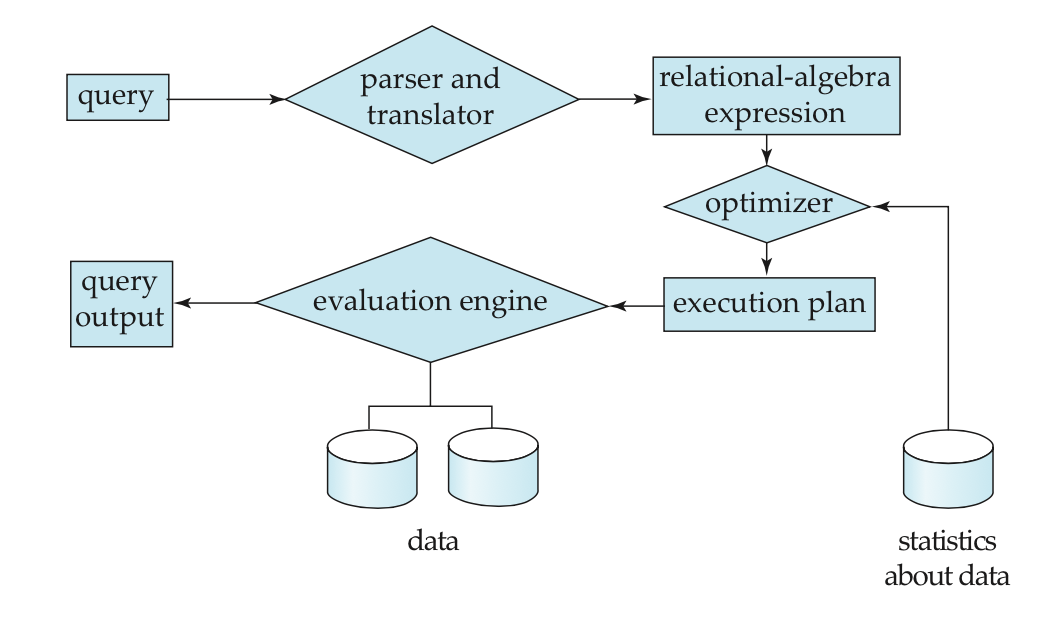
\includegraphics[width=\textwidth]{QueryProcessing}
	\caption{Steps in query processing~\cite{silberschatz2010database}.}
	\label{fig:qp}
\end{figure}

Once the execution plan has been produced, it is evaluated against the data stored in the database. If the query is one which accesses data, then output may be returned to the querying program; otherwise, there may be changes to the database's internal state~\cite{silberschatz2010database,harrington2009relational,garcia2000database}.

DeeBee's query processing system uses a simplified version of this general flow. For ease-of-implementation reasons, DeeBee interprets queries, rather than compiling and optimizing them. Furthermore, DeeBee's internal query representation takes the form of an abstract-syntax tree (AST) rather than a relational algebra expression. This is due to the fact that DeeBee does not implement the entire relational algebra, and some queries which DeeBee is capable of processing cannot be expressed in this manner.

\subsection{The Structured Query Language}
%-- new --%
SQL consists of two primary components, the \textit{Data Definition Language} or DDL, which is used to define the structures in which data is stored, and the \textit{Data Manipulation Language}, or DML, which is used for statements which access and modify the data stored in the database. The set of DDL statements which are run in order to create a database is referred to as the database's \texttt{schema}. A schema typically consists of a series of \texttt{CREATE TABLE} statements, which define each relation in the database by enumerating the names, data types, and constraints of each column in a table, as well as other statements, such as \texttt{CREATE TRIGGER}, which can be used to assign limited behaviors to various tables, and to create relationships between tables. Once a database has been created, it may be manipulated using DML statements such as \texttt{INSERT} to add data, \texttt{DELETE} to remove data, and \texttt{SELECT} to access data.

\subsubsection{DDL Grammar}

DeeBee's data definition language consists of the \texttt{CREATE TABLE} and \texttt{DROP TABLE} statements. Since DeeBee does not implement a number of advanced database features, such as the creation of triggers, the SQL constructs corresponding to those features have been removed. A Baukus-Naur Form for the DeeBee data definition language is given in \cref{lst:ddl-grammar}. Do note that in DeeBee SQL, as in many SQL dialects, keywords are not case sensitive; however, SQL keywords are conventionally typeset upper case.
\begin{listing}[h]
\begin{grammar}
<DDL-statement>  ::= <create-statement>
	 \alt <drop-statement>
	 
<create-statement> ::= `CREATE' `TABLE' <name> `(' <members> `)' `;'

<members> ::= <schema-item> `,' <column-list>
	\alt <schema-item>

<schema-item> ::= <attribute> \alt <referential-constraint> 	 
	
<attribute> ::= <name> <data-type> <constraint-list>

<constraint-list> ::= <attr-constraint> `,' <constraint-list>
	\alt <attr-constraint>
	
<attr-constraint> ::= `NOT' `NULL'  | `UNIQUE' | `PRIMARY' `KEY'

<data-type> ::= `INT'  | `INTEGER'  |`CHAR'  | `VARCHAR'  | `NUMERIC' | `DECIMAL'

<referential-constraint> ::= `FOREIGN` `KEY' `(' <names-list> `)' `REFERENCES'  <name> `(' <names-list> `)'

<names-list> ::= <name> `,' <names-list> \alt <name>

<delete-statement> ::= `DROP' `TABLE' <name> `;'
\end{grammar}
\caption{Grammar of DeeBee DDL statements}
\label{lst:ddl-grammar}
\end{listing}

In this grammar, the DeeBee DDL is defined as consisting of either \texttt{CREATE TABLE} or \texttt{DROP TABLE} statements.  A \texttt{CREATE TABLE} statement consists of the keyword \texttt{CREATE TABLE}, followed by the name of the table to be created, followed by a listing of the attributes and constraints placed on the table, surrounded by parentheses. Each attribute definition consists of a name, a type, and optional row constraints, such as \texttt{NOT NULL} or \texttt{UNIQUE}. \Cref{lst:create} provides an example of a \texttt{CREATE TABLE} statement. All valid SQL statements are terminated with the semicolon character.

\begin{listing}[h]
    \begin{minted}[gobble=8]{SQL}
        CREATE TABLE Writers (
            id           	  INTEGER NOT NULL PRIMARY KEY,
            first_name           VARCHAR(15) NOT NULL,
            middle_name          VARCHAR(15),
            last_name            VARCHAR(15) NOT NULL,
            birth_date           VARCHAR(10) NOT NULL,
            death_date           VARCHAR(10),
            country_of_origin    VARCHAR(20) NOT NULL
        );
\end{minted}
\caption{Example SQL \texttt{CREATE TABLE} statement.}
\label{lst:create}
\end{listing}

A \texttt{DROP TABLE} statement simply consists of the keywords \texttt{DROP TABLE} followed by the name of the table to be deleted. \Cref{lst:drop} provides an example of such a statement.

\begin{listing}[h]
    \begin{minted}[gobble=8]{SQL}
        DROP TABLE Writers;
\end{minted}
\caption{Example SQL \texttt{DROP TABLE} statement.}
\label{lst:drop}
\end{listing}

\subsubsection{DML Grammar}

DeeBee's data manipulation language consists of \texttt{SELECT}, \texttt{INSERT}, and \texttt{DELETE} statements. \texttt{INSERT} statements add rows to a table, while \texttt{DELETE} statements remove rows, and \texttt{SELECT} statements access rows. Most SQL implementations also include a \texttt{UPDATE} statement that modifies the data stored in table rows, but this statement was excluded from DeeBee as it is essentially syntactic sugar for actions that can be accomplished through the use of \texttt{DELETE} and \texttt{INSERT} statements. \Cref{lst:dml-grammar} presents a Baukus-Naur Form for the DeeBee DML.

\begin{listing}[h!]
\begin{grammar}
<DML-statement> ::= <select-statement> \alt <insert-statement> \alt <delete-statement>

<insert-statement> ::= `INSERT' `INTO' <name> `VALUES' `(' <vals-list> `)' `;'

<vals-list> ::= <literal> `,' <vals-list> \alt <literal>

<select-statement> ::= `SELECT' <projections> `FROM' <name> <where-clause> `;'

<projections> ::= <projection-list> \alt `*'

<projection-list> ::= <name> `,' <projection-list> \alt <name>

<where-clause> ::= `WHERE' <predicate> \alt $\varepsilon$

<predicate> ::= <comparison> <combining-op> <comparison> \alt <comparison>

<combining-op> ::= `AND'  |`OR'

<comparison> ::= <expr> <comparison-op> <expr>

<comparison-op> ::= `=' |`!=' | `<>' | `>=' | `<='  | `<' | `>'
\end{grammar}
\caption{Grammar of DeeBee DML statements.}
\label{lst:dml-grammar}
\end{listing}

\section{Implementation}

\subsection{The Scala Programming Language}

DeeBee was implemented using the Scala programming language, an object-oriented functional programming language which runs on the Java virtual machine~\cite{odersky2004scala,odersky2004overview,odersky2008programming}. Scala was designed by Martin Odersky of the Programming Methods Laboratory at \'Ecole Polytechnique F\'ed\'erale de Lausanne with the intention of developing a highly scalable programming language, ``in the sense that the same concepts can describe small as well as large parts''~\cite{odersky2004scala} and in the sense that Scala should be applicable to tasks of various sizes and complexities, and provide high performance at large scales~\cite{odersky2008programming}. 

Scala was inspired by criticisms of Java and by the recent popularity of functional programming langauges such as Haskell. It aims to provide a syntax that is more expressive than that of Java but is still readily accessable to Java programmers. It is a statically-typed language and was developed with a focus on type safety, immutable data structures, and pure functions~\cite{odersky2004scala,odersky2004overview,odersky2008programming}. Because it compiles to Java bytecode and runs on the JVM, Scala is mutually cross-compatible with Java, meaning that Scala code can natively call Java methods and use Java libraries, and vise versa~\cite{odersky2008programming}.

A key concept in the Scala design is the idea of an `embedded domain-specific language (DSL)'. Essentially, this concept suggests that Scala's syntax should be modifiable to the extent that code for specific tasks be expressed with its' own syntax within Scala. These DSLs are still Scala code and can still be compiled by the Scala compiler, but their syntax differs based on the task they are intended for~\cite{ghosh2010dsls,hofer2008polymorphic,odersky2008programming}. The Scala parsing library and the ScalaTest testing framework both provide exmaples of embedded DSLs.

Scala was chosen as the ideal language for DeeBee's implementation due to the expressiveness of its syntax, which allows complex systems to be implemented in few lines of code; its performance at scale; the existence of powerful libraries for text parsing and concurrent programming using the actors model; and the cross-platform capabilities of the JVM.

\subsection{Query Parsing}
DeeBee processes SQL queries by parsing the input query strings and generating an abstract syntax tree (AST) which represents the query. The AST is then interpreted against a context (typically a database or table) to determine the actions necessary to carry out the query. The query is then conducted using the API of the target relations to carry out the necessary operations.

DeeBee's query parser was implemented using the Scala standard library's combinator parsing ~\cite{moors2008parser} package. Combinator parsing is a method of parser implementation, popular in functional programming languages such as Scala and Haskell, which provides an alternative to parser generators such as \texttt{yacc} or \texttt{bison}.

In the parser generator approach, the grammar of a language is described using a syntax similar to Baukus-Naur Form (BNF), and then the parser generator is invoked on that grammar description. The parser generator uses the grammar description to produce the source code for a parser for that language\footnote{In the case of \texttt{bison}, these are LALR(1) parsers implemented in C}. This parser can be included in a project and used to parse text input. 

While the use of these tools is often much less demanding than implementing a parser by hand, the use of parser generators has a number of disadvantages. The generated source code is frequently highly complex and, since it is generated automatically, it may be poorly documented and difficult to understand. This can make debugging and maintaining the generated code very difficult.

\subsubsection{Combinator Parsing}

Combinator parsing provides a method of implementing recursive descent parsers using a BNF-like domain-specific language,  but rather than using that grammar description to generate parsing code, the grammar description is the source code of the parser, and can be inspected, maintained, and modified transparently~\cite{ghosh2010dsls,hofer2008polymorphic,moors2008parser}.

In this approach, a parser is defined as a function which takes as input a string and either accepts or rejects that string according to some rule. A parser combinator is a higher-order function which takes as parameters two parsers, and produces a new parser that combines the two input parsers. Parser combinators exist which combine the input parsers according to various rules, such as sequencing, alternation, optionality, or repetition. The language specification is written by repeatedly combining primitive parsers for tokens such as keywords, constants, and identifiers into more complex parsers for constructs such as expressions. At runtime, the parser then attempts to parse some input against the start symbol parser, which is composed of multiple smaller parsers, recursively descending through the grammar by calling each component parser.~\cite{moors2008parser,swierstra2001combinator,fokker1995functional,frost2008parser}

For example, in the Scala parser combinators library, the \texttt{\textasciitilde} parser combinator is the sequencing parser combinator. If \texttt{a} and \texttt{b} are parser functions, then the expression \texttt{a \textasciitilde b} would create a parser which accepts a string containing a substring accepted by \texttt{a} followed by a substring accepted by \texttt{b}. Similarly,  \texttt{|} is the alternation combinator, so the expression \texttt{a | b} specifies a parser that accepts either a string accepted by \texttt{a} or \texttt{b}.  The \texttt{.?} combinator can be applied to a single parser in order to make that parser optional (one or none), while the \texttt{.*} combinator will accept any number of repetitions of the input parser. 

Multiple parser combinators can be combined into complex expressions. For example, if \texttt{a}, \texttt{b}. and \texttt{c} are all parser functions, the expression \texttt{def d = a \textasciitilde b | c.*} defines \texttt{d} as a parser that accepts a string which contains a substring matching \texttt{a} followed by a substring matching either \texttt{b} or any number of repetitions of \texttt{c}.

\subsubsection{Packrat Parsing}
A major disadvantage of top-down parsers, such as the recursive descent parsers created through the use of parser combinators, is that they cannot parse left-recursive grammars. Scala's parsing library offers a solution to this problem by providing packrat parsing functionality.

Packrat parsing, first described by Bryan Ford in his masters' thesis~\cite{ford2002packrat} is a technique that both improves performance of backtracking parsers (such as recursive descent parsers), guaranteeing linear parse time, and allows the parsing of grammars containing left recursion, as well as any LL(\textit{k}) or LR(\textit{k}) language. Packrat parsing works by memoizing the results of each invocation of 

This class enhances parser combinators with the addition of a memoization facility. This allows recursive-descent parsing of left-recursive grammars. It also improves performance, providing linear-time parsing for most grammars~\cite{jonnalagedda2009packrat,ford2002packrat,ford2002packrat2}. I make liberal use of packrat parsers in order take advantage of their improved performance.

\subsubsection{Challenges}
Some difficulties were encountered in parsing, mostly related to the parsing of nested predicate expressions in SQL \texttt{WHERE} clauses. These issues were eventually resolved by separating the productions for `leaf' predicates (those consisting of a comparison between an attribute and an expression) and predicates consisting of multiple predicate expressions, and using the longest-match parser combinator to back-track in order to parse the entire \texttt{WHERE} clause.

\subsection{Query Interpretation}
\label{sec:query}
Queries are interpreted against a table using the \texttt{Relation} API. DeeBee defines a core trait for all tables, \texttt{Relation}, which defines a number of `primitive' operations on a table, such as filtering rows by a predicate, projecting a relation by selecting specific columns, and taking a subset number of rows. These in turn rely on two abstract methods, for accessing the table's attribute definitions and the set of the table's rows. These methods are implemented by each concrete class that implements \texttt{Relation}.

Relation is extended by two other traits, \texttt{Selectable} and \texttt{Modifyable}, which provide polymorphic functions for actually processing queries. These can be mixed in as needed to represent tables which support these functionalities.

Queries involving predicates, such as \texttt{SELECT} and \texttt{DELETE} statements with \texttt{WHERE} clauses, must go through an additional step of predicate construction, which converts SQL ASTs for \texttt{WHERE} clauses into Scala partial functions which take as a parameter a row from a table and return a Boolean. These functions are emitted by the AST node for \texttt{WHERE} clauses, using the target relation as a context for accessing the attributes corresponding to names in the SQL predicate. A similar process is performed for \texttt{INSERT} statements, which must be checked against the type and integrity constraints in the attribute corresponding to each value in the statement.

\section{Storage}
\label{sec:storage}
DeeBee currently provides one storage type, \texttt{CSVRelation}, which stores each table as a comma-separated values file on disk. While this storage mechanism is not ideal for a relational database, as it provides poor performance, it was used for the first DeeBee storage backend due to ease of implementation and testing. However, the DeeBee storage system is designed to be modular, making it possible to implement other storage backends in the future. I am considering the implementation of a B+ tree backend, similar to those used in `real-world' RDBMSs, and/or some form of hash bucket based storage.

\section{Further Research}
While DeeBee currently implements the entirity of the planned subset of SQL, there are a number of additional features that could be implemented. As discussed in \Cref{sec:storage}, CSV storage is not as performant as the storage methods used by real RDBMSs, and I am considering implementing a more advanced storage system. 

Furthermore, DeeBee SQL does not currently implement a large portion of SQL syntax, such as \texttt{JOIN}s, \texttt{UPDATE} statements, \texttt{VIEW}s, or aggregate functions such as \texttt{SUM} and \texttt{COUNT}. DeeBee also does not implement all of the data types available in other SQL databases, such as BLOBs (binary large objects) and CLOBs (character large objects). An implementation of the SQL \texttt{DATE} type based on \texttt{java.util.date} was prototyped but is currently not yet implemented. 

Finally, DeeBee's connections API, used by other programs to interact with the system, could be expanded with support for non-blocking connections and additional options to configure the connected database, similar to those available in the Java DataBase Connection driver (JDBC). I have considered the implementing a JDBC compatible API for DeeBee, but am not currently certain if this is possible, due to the differences between DeeBee and other SQL databases.
\pagebreak
\bibliography{assets/final}{}
\bibliographystyle{plain}

\end{document}